\chapter{Theory}
\section{The Operational Transconductance Amplifier}
The operational transconductance amplifier (OTA) is basically an op-amp without an output buffer. An OTA can be defined as an amplifier where all the nodes are low impedance except the input and output nodes. A schematic symbol of an OTA is shown in Figure.\ref{fig:OTA_symbol}. OTAs are generally programmable usually through the bias current that is provided to a differential amplifier. In the symbol, a bias voltage is being used as a programmable input. This bias voltage in turn controls the bias current of the amplifier. More on this later.

\begin{figure} [H]
\centering
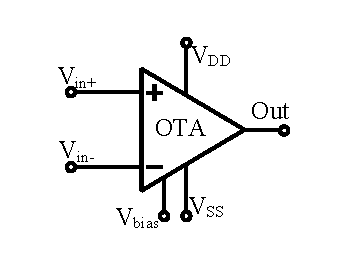
\includegraphics[scale=1]{Figures/System_Level/OTA_Symbol.pdf}
\caption{Symbol of an OTA}
\label{fig:OTA_symbol}
\end{figure}

\subsection{Conventional Current Mirror OTA}
The schematic of a conventional current mirror based OTA is as shown in Figure.\ref{fig:OTA_Schematic_Ibias}. The OTA employs a differential input pair in conjunction with three current mirrors. The differential input pair comprises of transistors $M_1$ and $M_2$. The differential pair is biased by the current mirror formed by $M_{nB1}$ and $M_{nB2}$. PMOS current mirrors formed by $M_3$, $M_5$ and $M_4$, $M_6$ reflect currents generated in the differential pair on to the output shell. The current generated by the mirror formed by $M_3$ and $M_5$ is reflected to the output via the NMOS currentn mirror formed by $M_7$ and $M_8$. The current mirror gain factor is K. Increase in K will increase the slew rate and gain bandwidth along with the output current of the conventional OTA at the cost of increased area, static power dissipation and a decrease in phase margin.

\begin{figure} [H]
\centering
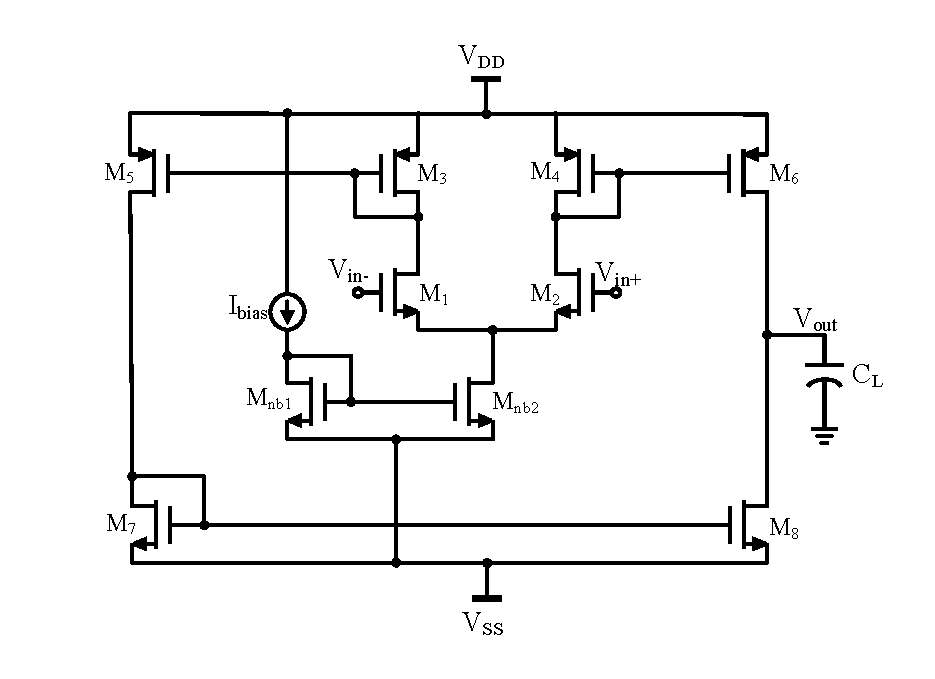
\includegraphics[scale=1]{Figures/Schematics/OTA_NMOS.pdf}
\caption{Schematic of a Conventional Current Mirror OTA}
\label{fig:OTA_Schematic_Ibias}
\end{figure}

Common mode signals are ideally rejected. i.e., when $V_{in+} = V_{in-}$, $I_{out}$ = 0. A differential input signal will generate an output current proportional to the applied differential voltage based on the transconductance of the differential pair. And that is why OTA is known as Voltage controlled Current Source. Although the output stage is push-pull structure, the conventional OTA is only capable for producing an output current with a maximum amplitude equal to the bias current in the output shell, provided the current mirror gain is unity, i.e., K=1. For this reason, conventional OTA is referred to as a Class A amplifier. 

The conventional OTA does not employ an output buffer and hence is only capable of driving capacitive loads and the capacitive load consumes all the current generated in the circuit. The gain of the OTA ($G_mR_o$) is dependent on the large output resistance of the output shell of the OTA formed by the transistors $M_3$ to $M_8$. The output resistance is reduced to $G_mR_o//R_L \approx G_mR_L$ if a parallel resistive load $R_L$ is applied.

Let us consider a hypothetical scenario that we do not need a resistive load to be driven as part of the system. In other words, we have a capacitive load as part of the specification. An advantage of this would be the fact that the need of an output buffer is eliminated and thereby the static power dissipation and the area occupied is reduced. But on the downside, the  amplifier behaviour for the output current would be like that of a band pass filter. So this scenario will not be useful as the specification demands a bandwidth of 10MHz as the overall system would be targetting low frequency applications. So a capacitive load will limit the output current only to a certain band of frequencies and hence it will not make sense to just use a one stage design. This gives rise to design an output buffer for the OTA.

An output buffer can either be a voltage buffer or a current buffer depending on how the OTA is designed. A current buffer, for example, is used to hold the output current of the OTA at the output of the buffer. So any amplification needed for this current would in turn give rise to the need of another stage, making the design complicated. In this case usually a current feedback amplifiers are designed which theoretically has a low input impedance non-inverting terminal input and a high input impedance inverting terminal input. So the OTA output would directly be connected to this non-inverting terminal and with the use of internal buffers, the output current follows the input current.

In this work, however, a voltage buffer amplifier is designed. Therefore, the OTA is used as a programmable block to control the output voltage rather than the output current.

\subsection{Other Topologies}
The Conventional OTA considered in the previous section is a Class A type of amplifier. These amplifiers can produce output currents that are equal to the bias currents for a unity current mirror gain. Need for high speed and high current with low power dissipation gave rise to research in Class AB Amplifiers. There are many topologies of the Class AB type OTAs that are classified based on their structure as:
\begin{itemize}
\item Folded Cascode OTA
\item Telescopic OTA
\item Local Common Mode Feedback OTA
\item Cascode Voltage Flipped Follower based OTA
\end{itemize}

One of the figures of merit to compare these OTAs is the Current Enhancement factor (CE). $CE = I_{out-max}/2I_{bias}$. Class A amplifiers typically have a CE of 1. Class AB OTAs have a high CE value. A family of OTA denoted as $Super Class-AB OTA$ have remarkably large CE values. Typical value of CE ranges from 100 to 500 depending on the implementation of the Class-AB differential pair and the output branches. Cascode Voltage Flipped Follower based OTA is one such example of a Super Class-AB OTA. These OTAs have the largest reported CE in literature.

\subsubsection{Super Class AB OTA}
The schematic of a Super Class AB OTA based on a Cascode Voltage Flipped Follower is as shown in Figure.\ref{fig:OTA_Class_AB}. It uses a Class-AB differential pair to boost the bias current by a factor of $k_1$. Typical values of $k_1$ range from 30 to 60 depending on the implementation of the Class-AB differential pair and supply voltages. An additional current boosting by a factor of $k_2$ is obtained in the output branches. The typical values of $k_2$ range from 3-8. Using cascode transistors maximum output current and subsequently the CE values are reduced. But lack of cascode transistors results in very low open loop gain. Therefore, a simple power efficient technique is used that allows the use of cascode transistors in order to achieve even higher open loop gain and gain bandwidth by maintaining a large CE value. This is done with the help of dynamically biasing the cascode transistors using RC networks (indicated in purple in the figure). The capacitor $C_{bat}$ acts as a floating battery for dynamic operations that transfers variations in the gate voltages of mirror transistors to the gate of the cascode transistors. This increases the $V_{DS}$ of the mirror transistors allowing high output currents. Cascode Voltage Flipped Follower (indicated in red in the figure) is charaterized by high input swing and can operate over a wide range of supply voltages. It uses local shunt feedback to provide nodes A and B with very low impedance.

\begin{figure} [H]
\centering
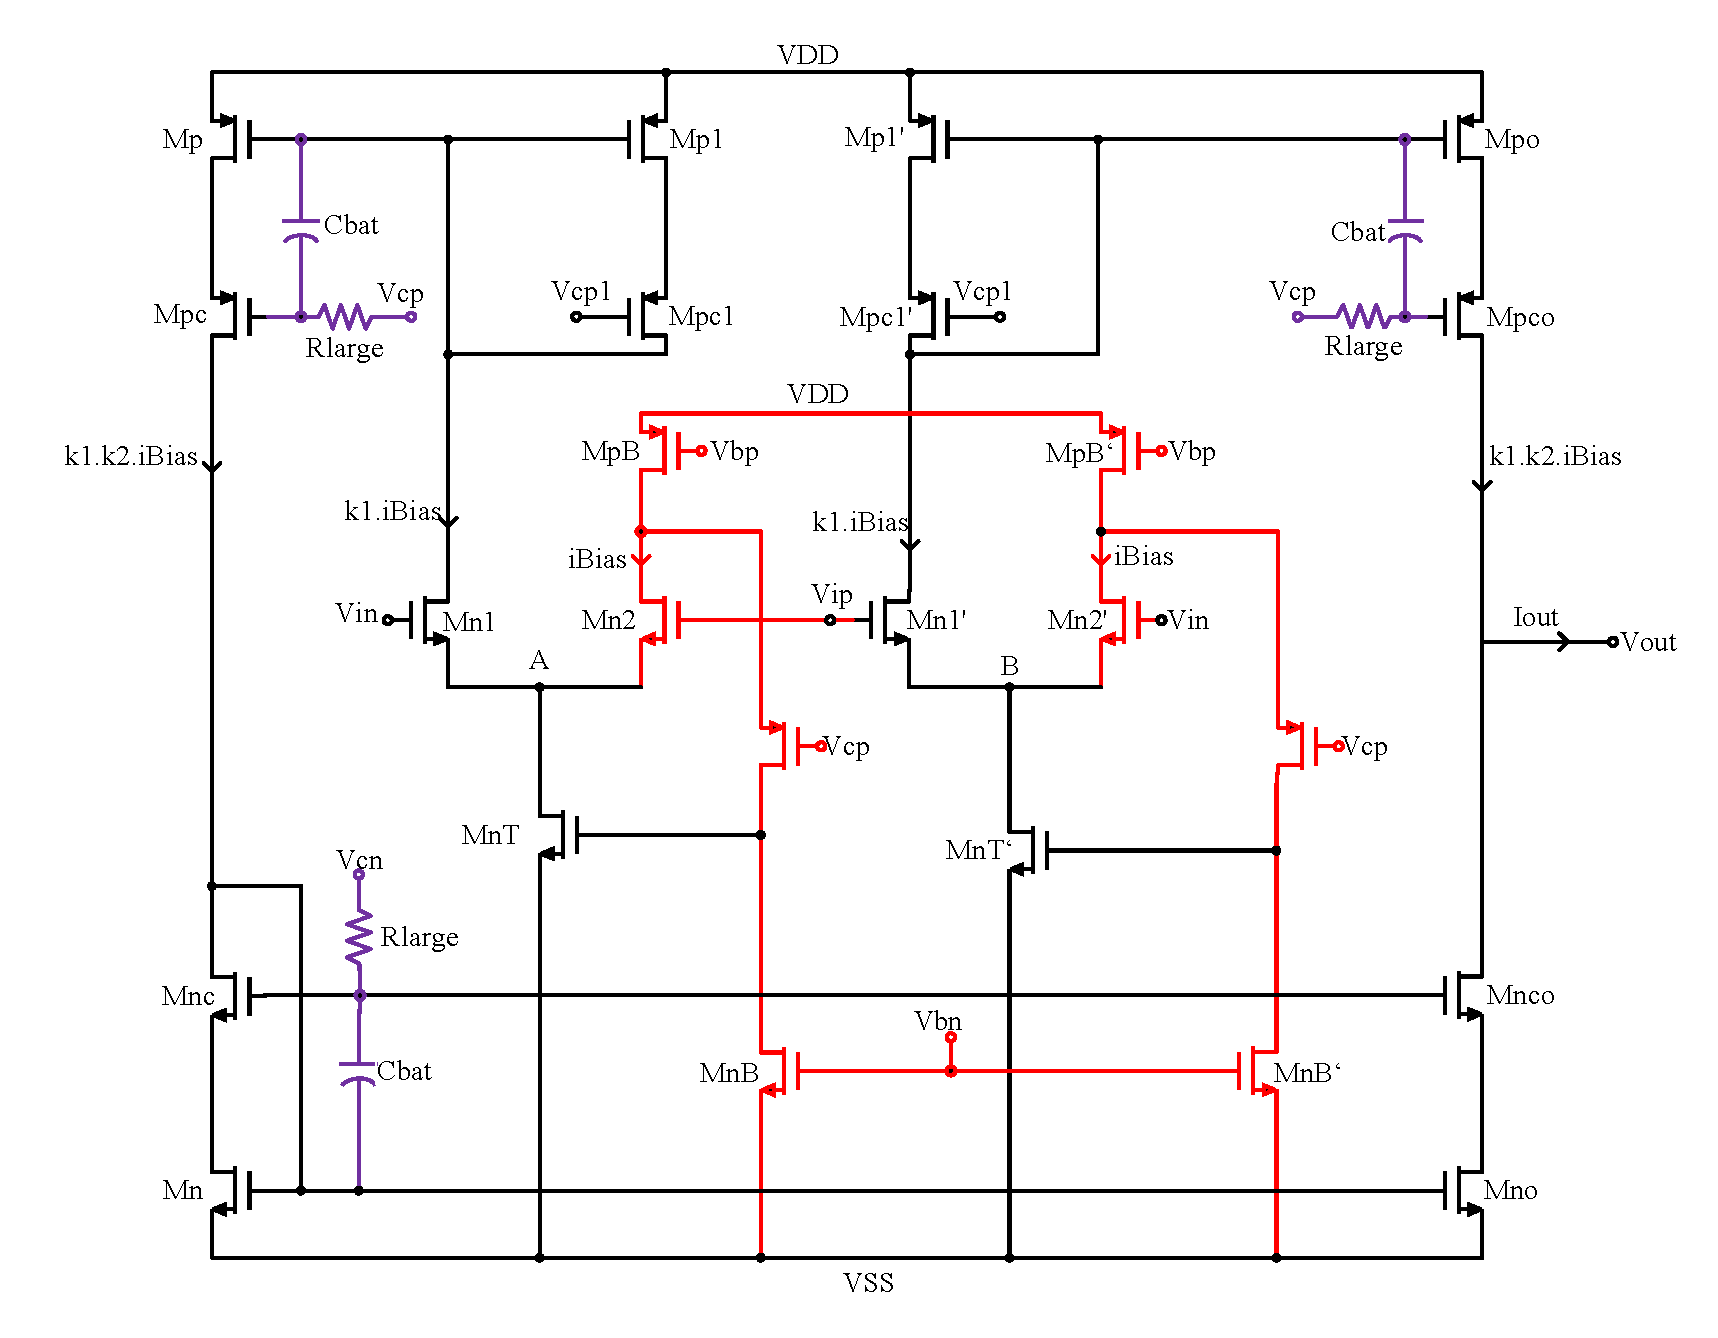
\includegraphics[scale=0.65]{Figures/Misc/OTA_Class_AB.pdf}
\caption{Super Class-AB OTA with a Cascode Voltage Flipped Follower}
\label{fig:OTA_Class_AB}
\end{figure}

Taking into account the complexity, output current requirements and load requirements, this design will not be considered further as part of this research work. The reason being - a high current output of this Class AB OTA would give rise to another output buffer. And the capacitors needed to consume such a high current would be in the order of several pico Farads. Having such a big capacitor inside an IC is not recommended. Also, considering how complex CMOS Current Feedback Amplifiers are, it is wise to stick to a simpler design that does the same work but with some minor trade-offs.
\vfill
\clearpage

\section{The Opeartional Amplifier}
The operational amplifier (OP AMP) is a fundamental building block in analog integrated circuit design. A typical symbol of an OP AMP is as shown in Figure.\ref{fig:OPAMP_symbol}. It consists of differential input terminals - inverting ($V_{in-}$) and non-inverting ($V_{in+}$), a positive supply pin ($V_{DD}$) and a negative/ground supply pin ($V_{SS}$) and the output terminal ($V_{out}$). Simple OP AMPs are generally used as Summing amplifier, differentiator, integrator, transimpedance amplfier, and so on. OP AMPs with vastly different levels of complexity are used to realize functions ranging from dc bias generation to high-speed amplification or filtering.

\begin{figure} [H]
\centering
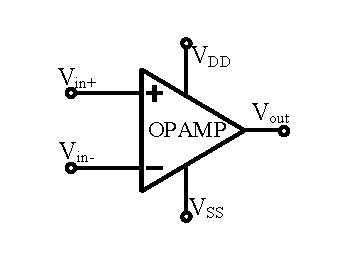
\includegraphics[scale=1]{Figures/System_Level/OPAMP_Symbol.pdf}
\caption{Symbol of an OP AMP}
\label{fig:OPAMP_symbol}
\end{figure}

OP AMPs are voltage controlled voltage sources, much to the contrary of OTAs, which are voltage controlled current sources. Design of an OP AMP consists of determining the specifications, selecting the device sizes and biasing conditions, compensating the op-amp for stability, simulating and characterizing the open loop gain, the input common mode range, common mode rejection ratio, power supply rejection ration, output votlage range, current sourcing/sinking capability and power dissipation.
OP AMPs are used as a voltage buffer whenever there is a need to drive resistive loads or a combination of capacitive load and a resistive load.

\subsection{Miller Compensation OP AMP}
The schematic of the a two-stage Miller Compensation OP AMP is as shown in Figure.\ref{fig:OPAMP_Schematic_Ibias}. First stage of the OP AMP is the differential amplfier formed by the transistors $M_1-M_5$ and $M_8$. The second stage of the OP AMP is the Common Source amplifier formed by the transistors $M_6$ and $M_7$. Compensation Capacitor or Miller Capacitor denoted by $C_C$ is used for the splitting of the poles of the two stages thereby providing stability and also controlling the bandwidth and the slew rate. 
\begin{figure} [H]
\centering
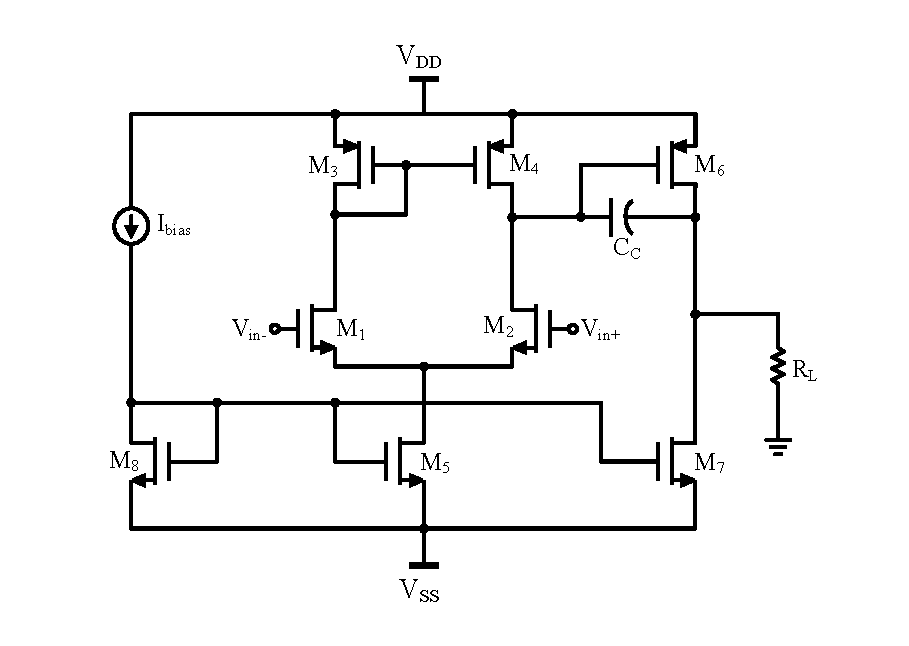
\includegraphics[scale=1]{Figures/Schematics/OPAMP_Ibias.pdf}
\caption{Schematic of a Two-stage Miller Compensation OP AMP}
\label{fig:OPAMP_Schematic_Ibias}
\end{figure}
The biasing to the differential input pair is provided by the current mirror formed by $M_5$ and $M_8$. The selection of the bias current, $I_{bias}$ is determined by gain, ICMR, CMRR, power dissipation, noise, slew rate and matching considerations. If slew-rate is of concern, a cross-coupled differential amplifier should be considered for the first stage. The second stage common source amplifier is used to provide an additional gain to the overall OP AMP since the gain provided by the differential pair is usually not large enough. It is known that OP AMPs have infinitely large open loop gain. This second stage also provided a current boosting since $M_7$ forms a current mirror with $M_8$ and the dimensions of $M_7$ are usually larger than $M_8$, thereby setting the current at the output of the OP AMP. The best use of these OP AMPs are made as part of voltage buffers. i.e., the OP AMP is connected in unity gain configuration by providing a direct feedback from the output terminal to the non-inverting terminal.
\vfill
\clearpage
\section{The Gm/Id Methodology}
